\subsection{Serveur local}


\subsubsection{Infrastructure}
Il y a trois serveurs locals chez Data-Gest. 
\begin{itemize}
\item[•]DATAGESTSRV01: Il y a trois missions principales de ce serveur. Tous d'abord, il gère tous les sessions de chaque utilisateur de DATA GEST. Ensuite, il sert à un serveur de SMB, à fin de partager les fichiers et les ressources entre différent département. En plus, il est aussi un serveur de FTP.  
\item[•]DATAGESTSRV02: C'est un serveur mail(EX-change 2010) avec système exploitation de WINDOWS. Il stocke tous les histoire et les data de mail de chaque session. 
\item[•]SRV-NAVISION: Toutes les informations, les flux, les commande, les listes de cadeaux sont envoyés à ce serveur pour traiter.
\end{itemize}




\subparagraph{}
L'infrastructure est déjà configurée en mode failover. C'est à dire que l'ip sur lequel le service est hébergé est routé sur le
serveur princial (ns26393.ovh.net). En cas de panne du serveur principale l'adresse ip est routée vers le serveur
secondaire. Par conséquent il faudra configurer les domaines de production pour qu'ils dirigent vers l'adresse IP
178.33.251.180.




%\begin{itemize}
%\item Liste a puces 1
%			\begin{itemize}
%			\item Liste a puces 2
%						\begin{itemize}
%						\item Liste a puces 3
%						\end{itemize}
%			\end{itemize}
%\end{itemize} 
%
%\paragraph{Titre de niveau 4}
%Non ergo erunt homines deliciis diffluentes audiendi, si quando de amicitia, quam nec usu nec ratione habent cognitam, disputabunt.
%
%\begin{figure}[H]
%	\center
%	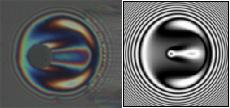
\includegraphics[width=5cm]{body/images/figure_example.png} 
%	\caption{Exemple de figure avec légende}
%	\label{fig:exemple}
%\end{figure}
%
%\subparagraph{Titre de niveau 5}
%
%Isdem diebus Apollinaris Domitiani gener, paulo ante agens palatii Caesaris curam, ad Mesopotamiam missus a socero per militares numeros immodice scrutabatur, an quaedam altiora meditantis iam Galli secreta susceperint scripta, qui conpertis Antiochiae gestis per minorem Armeniam lapsus Constantinopolim petit exindeque per protectores retractus artissime tenebatur.
%
%Titre de niveau 6
%Non ergo erunt homines deliciis diffluentes audiendi,


